\documentclass{jib}
\newlength{\platz}
\setlength{\platz}{15pt}
\RequirePackage{listings}
\lstset{%
  basicstyle=\ttfamily,
  fontadjust,
  flexiblecolumns=true,
  frame=L,
  xleftmargin=15pt,
  framesep=5pt,
  emphstyle=\rmfamily\itshape}

\usepackage{pdfpages}

%%%%%%%%%%%%%%%%%%%%%%%%%%%%%%%%%%%%%%%%%%%%%%%%%%%%%%%%%%
% JIB Header/Footer
%%%%%%%%%%%%%%%%%%%%%%%%%%%%%%%%%%%%%%%%%%%%%%%%%%%%%%%%%%
\jibvolume{XX} % insert volume
\jibissue{X}   % insert issue
\jibpages{XXX} % insert article ID
\jibyear{XXXX} % insert year
\makeHeaderFooter{} % leave as is
%%%%%%%%%%%%%%%%%%%%%%%%%%%%%%%%%%%%%%%%%%%%%%%%%%%%%%%%%%

\begin{document}

%%%%%%%%%%%%%%%%%%%%%%%%%%%%%%%%%%%%%%%%%%%%%%%%%%%%%%%%%%
%
% Title Page
%
%%%%%%%%%%%%%%%%%%%%%%%%%%%%%%%%%%%%%%%%%%%%%%%%%%%%%%%%%%

\begin{jibtitlepage}

\jibtitle{SBML Level 3 Package:\\
Spatial Processes, Version 1, Release 1}


% Please make sure to use unique footnote characters for each author
\jibauthor{%
  James C. Schaff\iref{uconn},
  Anuradha Lakshminarayana\iref{uconn},
  Robert F. Murphy\iref{mellon},
  Frank T. Bergmann\iref{heidelberg},
  Akira Funahashi\iref{keio},
  Devin P. Sullivan\iref{kth},
  Lucian P. Smith\iref{uw},
}

%\addjibinstitution{imbio}{IMBio, Ralf Hofest\"adt, Bielefeld University, Faculty of Technology, Bioinformatics Department, D-33501 Bielefeld, Germany, \url{http://www.imbio.de}}
\addjibinstitution{uconn}{University of Conneticut, US}
\addjibinstitution{mellon}{Carnegie Mellon University, US}
\addjibinstitution{heidelberg}{University of Heidelberg, DE}
\addjibinstitution{keio}{Keio University, JP}
\addjibinstitution{kth}{KTH-Royal Institute of Technology, SE}
\addjibinstitution{uw}{University of Washington, US}



\end{jibtitlepage}


% adjusts the width of the abstract, please do not change!
%\begin{adjustwidth}{}{1cm} %LS NOTE:  'adjustwidth' not recognized in my setup.

\renewcommand{\baselinestretch}{1.0}
\abstract{While many biological processes can be modeled by abstracting away the space in which those processes occur, some modeling (particularly at the cellular level) requires space itself to be modeled, with processes happening not in well-mixed compartments, but spatially-defined compartments.  The \emph{SBML Level~3 Core} specification does not include an explicit mechanism to encode geometries and spatial processes in a model, but it does provide a mechanism for SBML \emph{packages} to extend the Core specification and add additional syntactic constructs. The SBML \emph{Spatial Processes} package for SBML Level~3 adds the necessary features to allow models to encode geometries and other spatial information about the elements and processes it describes.}

%\end{adjustwidth} % please do not change %LS NOTE:  'adjustwidth' not recognized in my setup.


% Include your PDF document
\clearpage
\setlength{\voffset}{0cm}
\setlength{\hoffset}{0cm}
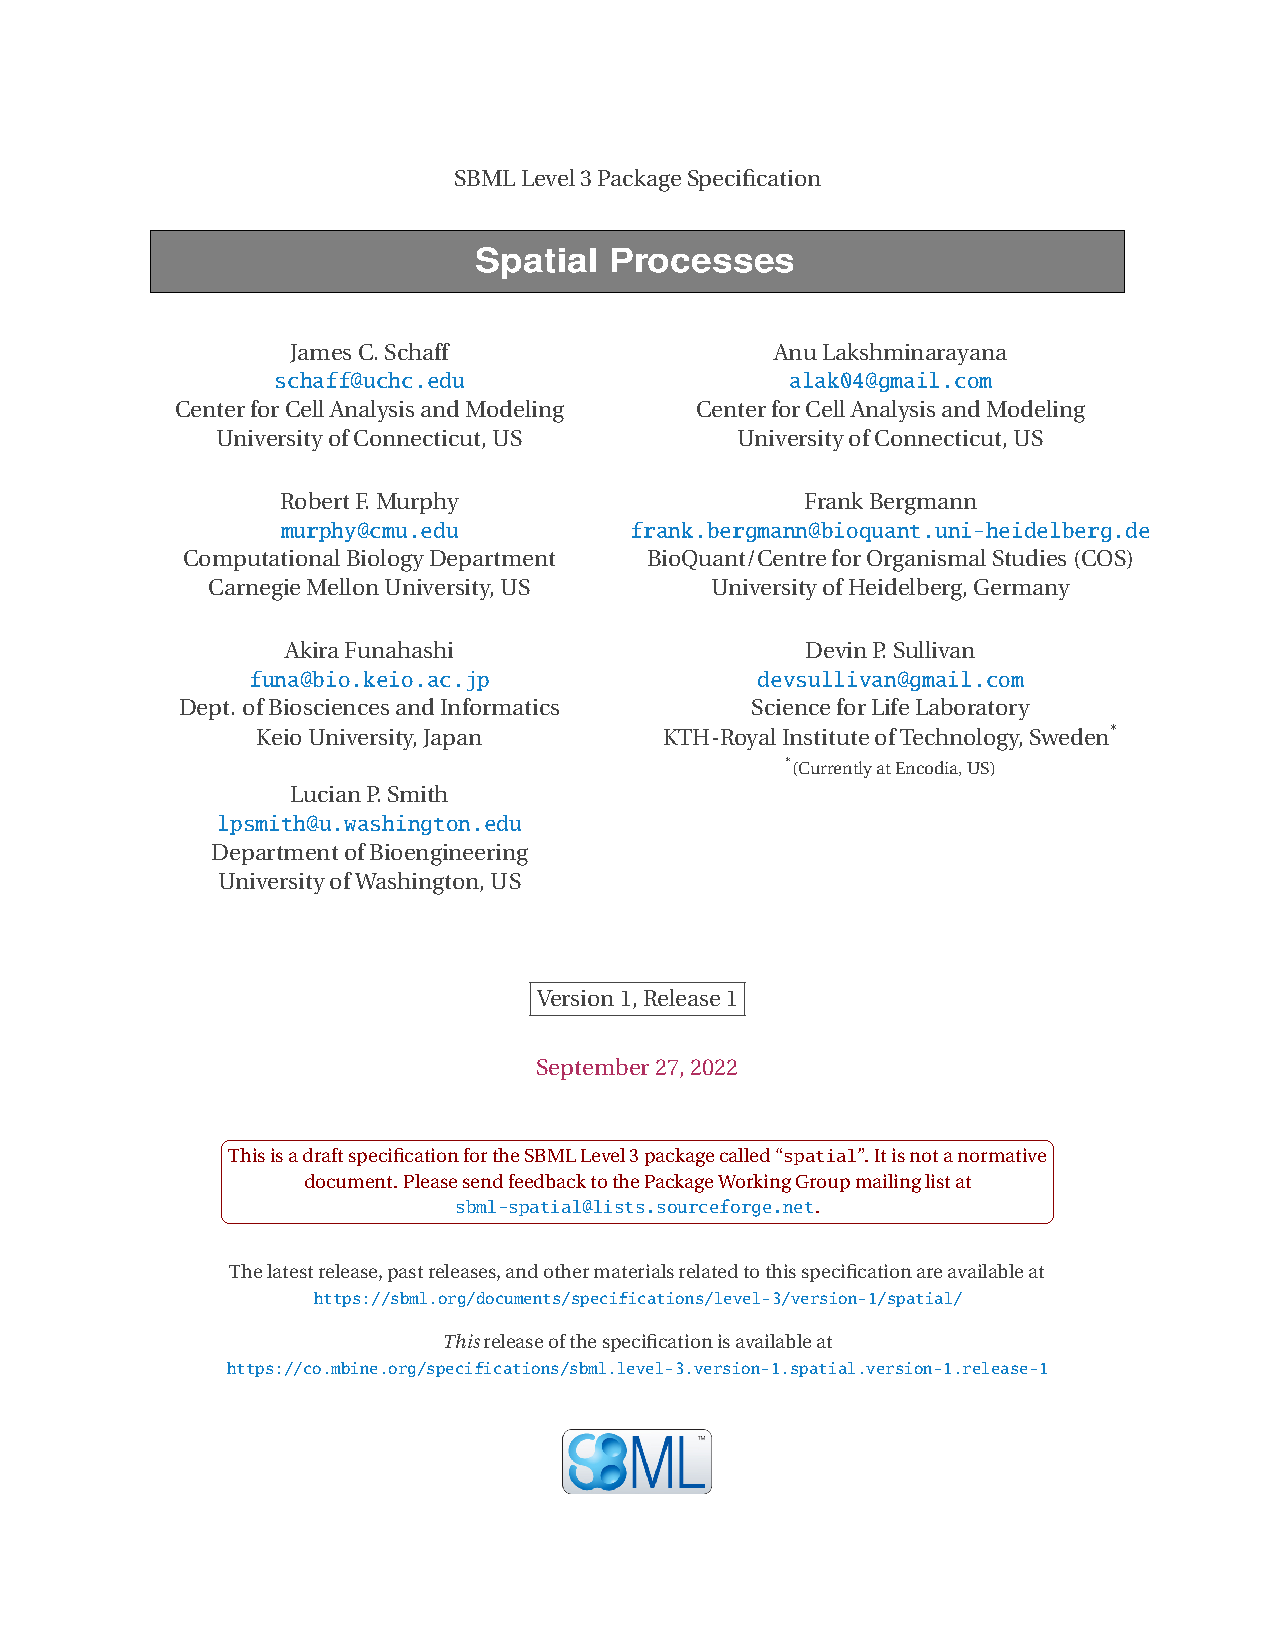
\includepdf[pages=-]{sbml.level-3.version-1.spatial.version-1.release-1.pdf}

\end{document}
